% Copyright (C) 2012 Shi.Zhan <g.shizhan.g@gmail.com>
%
% Permission is hereby granted, free of charge, to any person obtaining a copy of this software and associated documentation files (the "Software"), to deal in the Software without restriction, including without limitation the rights to use, copy, modify, merge, publish, distribute, sublicense, and/or sell copies of the Software, and to permit persons to whom the Software is furnished to do so, subject to the following conditions:
%
% The above copyright notice and this permission notice shall be included in all copies or substantial portions of the Software.
%
% THE SOFTWARE IS PROVIDED "AS IS", WITHOUT WARRANTY OF ANY KIND, EXPRESS OR IMPLIED, INCLUDING BUT NOT LIMITED TO THE WARRANTIES OF MERCHANTABILITY, FITNESS FOR A PARTICULAR PURPOSE AND NONINFRINGEMENT. IN NO EVENT SHALL THE AUTHORS OR COPYRIGHT HOLDERS BE LIABLE FOR ANY CLAIM, DAMAGES OR OTHER LIABILITY, WHETHER IN AN ACTION OF CONTRACT, TORT OR OTHERWISE, ARISING FROM, OUT OF OR IN CONNECTION WITH THE SOFTWARE OR THE USE OR OTHER DEALINGS IN THE SOFTWARE.
%
% 课程:人机交互技术及应用
% 班级:传播学1001班
% 课时:40学时,2012年秋季1~10周,每周一、三
% 地点:东九楼D212
% 主页:http://code.google.com/p/hci-course/
% 教师:施展 
% 单位:华中科技大学 武汉光电国家实验室
%
\documentclass{beamer}
\usepackage{fontspec,xunicode,xltxtra,beamerthemesplit}
%\usetheme{Hannover} % White background
\usetheme{Berkeley} % Blue background
\setmainfont[
	BoldFont={WenQuanYi Zen Hei},
	ItalicFont={WenQuanYi Micro Hei}
]{WenQuanYi Micro Hei}
\setsansfont[
	BoldFont={WenQuanYi Zen Hei},
	ItalicFont={WenQuanYi Micro Hei}
]{WenQuanYi Micro Hei}

% 中文环境自动换行
\XeTeXlinebreaklocale "zh"
\XeTeXlinebreakskip = 0pt plus 1pt

% 中文环境修正导航栏
\makeatletter
\def\beamer@linkspace#1{
	\begin{pgfpicture}{0pt}{-1.5pt}{#1}{5.5pt}
		\pgfsetfillopacity{0}
		\pgftext[x=0pt,y=-1.5pt]{.}
		\pgftext[x=#1,y=5.5pt]{.}
	\end{pgfpicture}
}
\makeatother

%% diagrams
%\usepackage{tikz}
%\usetikzlibrary{arrows,shapes}
%
%% full page image
%\newcommand{\fullPageImage}[2]{
%	{
%		\usebackgroundtemplate{\includegraphics[width=\paperwidth, height=\paperheight]{#1}}
%		\frame[plain]{#2}
%	}
%}

\title{人机交互技术}
\author{施展}
\institute{华中科技大学~武汉光电国家实验室}
\date{\today}
\titlegraphic{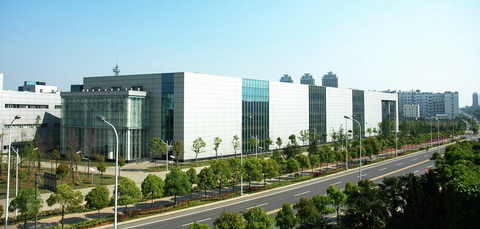
\includegraphics[width=2cm]{images/wnlo.jpg}}

\begin{document}

\begin{frame}
	\titlepage
\end{frame}

\begin{frame}
	\frametitle{内容提要}
	\tableofcontents
\end{frame}

\section{第八讲}
\begin{frame}
	\frametitle{第八讲 移动界面设计}
	本章主要目的:
	\begin{itemize}
		\item 课堂研讨
		\begin{itemize}
			\item 移动平台界面特点及感受
			\item 移动平台主要技术之一二
			\item 移动平台APP+Web及今后
%			\item 给出移动界面设计实例
		\end{itemize}
	\end{itemize}
\end{frame}

\subsection{移动平台界面特点}
\begin{frame}
	\frametitle{移动平台界面特点及感受}
	\begin{itemize}[<+->]
		\item 小、快、灵
		\item 多通道
	\end{itemize}
\end{frame}

\subsection{移动平台主要技术}
\begin{frame}
	\frametitle{移动平台主要技术之一二}
	\begin{itemize}[<+->]
		\item 二个半大平台/生态环境
		\begin{itemize}
			\item 谷歌 Android
			\item 苹果 IOS
			\item 以及东山再起的微软 Windows Phone
		\end{itemize}
		\item 塞班 Symbian 已成为过去
		\item 接班人 MeeGo \dots
		\item 新兴的平台 Firefox OS?
		\item Linux?
	\end{itemize}
\end{frame}

\subsection{移动应用与Web}
\begin{frame}
	\frametitle{移动应用与Web}
	\begin{itemize}
	\item 传统APP VS. HTML 5
	\end{itemize}
\end{frame}

%\subsection{移动界面设计实例}
%\begin{frame}
%	\frametitle{移动界面设计实例}
%
%\end{frame}

\section{小结}
\begin{frame}
	\frametitle{小结}
	\begin{itemize}
		\item 了解、认识移动界面及相关概念、关键技术及工具
		\item 探讨移动界面设计原则、基本要素
	\end{itemize}
\end{frame}

\end{document}